%%%%%%%%%%%%%%%%%%%%%%%%%%%%%%%%%%%%%%%%%
% Short Sectioned Assignment
% LaTeX Template
% Version 1.0 (5/5/12)
%
% This template has been downloaded from:
% http://www.LaTeXTemplates.com
%
% Original author:
% Frits Wenneker (http://www.howtotex.com)
%
% License:
% CC BY-NC-SA 3.0 (http://creativecommons.org/licenses/by-nc-sa/3.0/)
%
%%%%%%%%%%%%%%%%%%%%%%%%%%%%%%%%%%%%%%%%%

%----------------------------------------------------------------------------------------
%	PACKAGES AND OTHER DOCUMENT CONFIGURATIONS
%----------------------------------------------------------------------------------------

\documentclass[paper=a4, fontsize=11pt]{scrartcl} % A4 paper and 11pt font size
\usepackage[margin=1in]{geometry}

\usepackage[T1]{fontenc} % Use 8-bit encoding that has 256 glyphs
\usepackage{fourier} % Use the Adobe Utopia font for the document - comment this line to return to the LaTeX default
\usepackage[english]{babel} % English language/hyphenation
\usepackage{amsmath,amsfonts,amsthm} % Math packages
\usepackage{float}

\usepackage{lipsum} % Used for inserting dummy 'Lorem ipsum' text into the template

\usepackage{sectsty} % Allows customizing section commands
\allsectionsfont{\centering \normalfont\scshape} % Make all sections centered, the default font and small caps

\usepackage{fancyhdr} % Custom headers and footers
\pagestyle{fancyplain} % Makes all pages in the document conform to the custom headers and footers
\fancyhead{} % No page header - if you want one, create it in the same way as the footers below
\fancyfoot[L]{} % Empty left footer
\fancyfoot[C]{} % Empty center footer
\fancyfoot[R]{\thepage} % Page numbering for right footer
\renewcommand{\headrulewidth}{0pt} % Remove header underlines
\renewcommand{\footrulewidth}{0pt} % Remove footer underlines
\setlength{\headheight}{13.6pt} % Customize the height of the header

\numberwithin{equation}{section} % Number equations within sections (i.e. 1.1, 1.2, 2.1, 2.2 instead of 1, 2, 3, 4)
\numberwithin{figure}{section} % Number figures within sections (i.e. 1.1, 1.2, 2.1, 2.2 instead of 1, 2, 3, 4)
\numberwithin{table}{section} % Number tables within sections (i.e. 1.1, 1.2, 2.1, 2.2 instead of 1, 2, 3, 4)

\usepackage{parskip}
\setlength\parindent{0pt} % Removes all indentation from paragraphs - comment this line for an assignment with lots of text

\usepackage{graphicx}
\graphicspath{ {images/} }

%----------------------------------------------------------------------------------------
%	TITLE SECTION
%----------------------------------------------------------------------------------------

\newcommand{\horrule}[1]{\rule{\linewidth}{#1}} % Create horizontal rule command with 1 argument of height

\title{	
\normalfont \normalsize 
\textsc{CMSC 312} \\ [25pt] % Your university, school and/or department name(s)
\horrule{0.5pt} \\[0.4cm] % Thin top horizontal rule
\huge Operating System Simulator Project \\ % The assignment title
\horrule{2pt} \\[0.5cm] % Thick bottom horizontal rule
}

\author{Paul Hudgins, Emily Klein, Quark Wei%} % Your name
\\ \normalsize V70270484, V00374656, V00687866}

\date{\normalsize November 29, 2016}%\today} % Today's date or a custom date

\begin{document}

\maketitle % Print the title

%----------------------------------------------------------------------------------------
%	PROBLEM 1
%----------------------------------------------------------------------------------------

The Operating System Simulator runs with a memory limitation of 256kB, handles six traps and interrupts, and implements both a short-term and long-term scheduler with priorities and aging. The simulator simulates processes that compete for resources such as the CPU and I/O. I/O access is controlled but mutex locks and device queues that prevent busy waiting.

 The simulator features a terminal emulator with auto-complete, command history, and a limited implementation of the `cat' shell command. The GUI also as visuals to help the user understand the current state of the simulator.

\section{Usage}

 All job and program files must be placed in the \textit{Program Files} directory to be used, and must have the file extensions \textit{.prgrm} and \textit{.job}, respectively.

The command line interface will auto-suggest while you type. Suggestions can be completed by pressing the Tab key. The previous command can be repeated by pressing the Enter key. All previous commands can be accessed with the Up arrow.

The \textit{LOAD} command is used to load \textit{jobs} and \textit{programs}, allowing for multiple inputs/parameters at a time, but is also used to list all loadable files if no parameters are passed in.

The command-line interface implements most features of cat, which allows for redirection into an output file. This means you can create and view the contents of program and job files on-the-fly.

\subsection{shortTermSchedulerTest.job}
The following features can be observed when running shortTermSchedulerTest.job.
\begin{itemize}
	\item The most CPU time is given to a High\_Priority\_CPU\_Bound\_Process.
	\item IO utilization is indicated by a process being in the pink WAIT\_FOR\_IO state. Utilization is higher than would be expected based on priorities and aging alone. This is because a waiting process is given preference for the burst after the IO device is released. Frequently, a process can be observed in the WAIT\_FOR\_IO state with an aged priority of 1 or 0, which is lower than the high-priority process' base priority of 2.
	\item The Low\_Priority\_Background process receives the least CPU time, but does not undergo starvation.
\end{itemize}

\subsection{longTermSchedulerTest.job}
The following features can be observed when running longTermSchedulerTest.job.
\begin{itemize}
	\item Memory usage never exceeds 256kb. Processes that are in the Orange STANDBY or White NEW states consume memory on the backing store, but not in main memory.
	\item The long-term scheduler is executed at least once for every 20 cycles of the short term scheduler. Execution of the long-term-scheduler can be observed when there is a change in which processes are in the Orange STANDBY state.
	\item Processes that have not yet been executed are given an age based on the start-time of the system. Ensures that new processes have the highest priority, and are swapped into memory first.
\end{itemize}


\section{Simulation Architecture}

The simulator consists of three main packages. The \textit{simulator} package simulates hardware operation, including CPU execution and IO. The \textit{kernel} package contains the operating system which controls the simulated hardware. The \textit{user\_interface} package contains the shell and GUI.


\subsection{Compiler and Critical Sections}
The Compiler in the \textit{utilities} package reads program files and compiles them into an array of Operation objects, which are machine code instructions for our simulator. In addition to creating the appropriate parameters for CALCULATE operations, the Compiler will also insert an ACQUIRE operation before and a RELEASE operation after each IO operation, creating a critical section in the code. When a process is executing in its critical section, no other process will be able to acquire the IO device in use.

\subsection{Execution}
Because the CALCULATE operation consumes a variable number of cycles, the CPU uses an Operation Counter as well as a Program Counter. The Program Counter, as usual, indicates which operation is currently being executed, and the Operation Counter indicates how many cycles are remaining for that operation.
Because kernel methods are executed on the JVM and not on the simulated processor, kernel methods do not consume CPU cycles. All operations on the simulated CPU can be considered to execute in ``user mode'' and all methods from the \textit{kernel} package can be considered to execute in ``kernel mode''. The only way to go from user mode to kernel mode is to signal an interrupt.

\subsection{Interrupts}

The hardware will blindly continue execution of the current process in user mode until an interrupt flag is set in the interrupt processor. The interrupt processor then routes the interrupt to the appropriate handler. Most interrupt handlers will make use of a common context-switch handler which copies CPU registers to the PCB for the current process and copies saved register states from the next PCB to the CPU. All interrupts are preemptive. The interrupt processor supports two system-driven interrupts and four traps:


\begin{itemize}
	\item YIELD: Triggered by expiration of the burst timer set by the short term scheduler
          \item IO\_COMPLETE: Signals that an IO event needs to be handled
           \item TERMINATE: Terminates the current process
	\item ACQUIRE: Requests access to a resource, blocking if the resource is not available, so that busy waiting is avoided
	\item RELEASE: Releases a resource
	\item WAIT\_FOR\_IO: Blocks until an IO\_COMPLETE signal is received
\end{itemize}

\section{Scheduling}

The system uses a short-term scheduler and a long-term scheduler. The short-term scheduler executes at the end of every CPU burst. The long-term scheduler executes after 20 calls to the short-term scheduler, or if the short-term scheduler is unable to select a process for execution.

\subsection{Short-term Scheduler}

The short-term scheduler schedules CPU bursts and IO for processes that are in memory. It utilizes the following queues:
\begin{itemize}
	\item Ready Queue: There is one priority queue of processes waiting for CPU time.
           \item Device Queues: There is one queue of processes waiting for accesses for each IO device. 
Currently, the simulation only uses one IO device, but it can accommodate more. When one process releases
a device, the short-term scheduler immediately attempts to execute another process waiting for that device in order to
maximize IO utilization.
	\item Waiting Queue: There is one queue of processes waiting for a signal. Because IO response is the only signal in the
simulator, there is no Event Queue. The running process will be preempted and the waiting process will be executed as soon as a signal is received.

\end{itemize}

\subsection{Long-term Scheduler}

The long-term scheduler swaps processes in and out of memory, ensuring that the memory limit is not exceeded. Each time the long-term scheduler executes, it does the following:
\begin{itemize}
	\item Pulls all new processes off of the New Process Queue
           \item If space is available in memory, processes from the Standby Queue are swapped into memory until there is no more space available.
	\item If processes remain in Standby Queue, some processes are swapped out of memory to make room for processes that are standing by.

\end{itemize}

\subsection{Scheduling Algorithm}
Both the long-term scheduler and short-term scheduler use highest-priority first, with aging. Each program can be assigned a priority in the second line of the program file, with the command PRIORITY and an integer argument. Scheduling queues are implemented as priority heaps. The effective priority of a process is its base priority plus one fiftieth of its age. Age is defined as the time since the end of the last CPU burst. 

To maximize IO utilization, the RELEASE handler will immediately schedule the next process waiting for the device, even if there are higher priority processes in the waiting queue. This gives the IO-bound process one ``free'' CPU burst, so that it can attempt to enter a state where it is waiting for a response signal from the IO device.

\section{GUI}
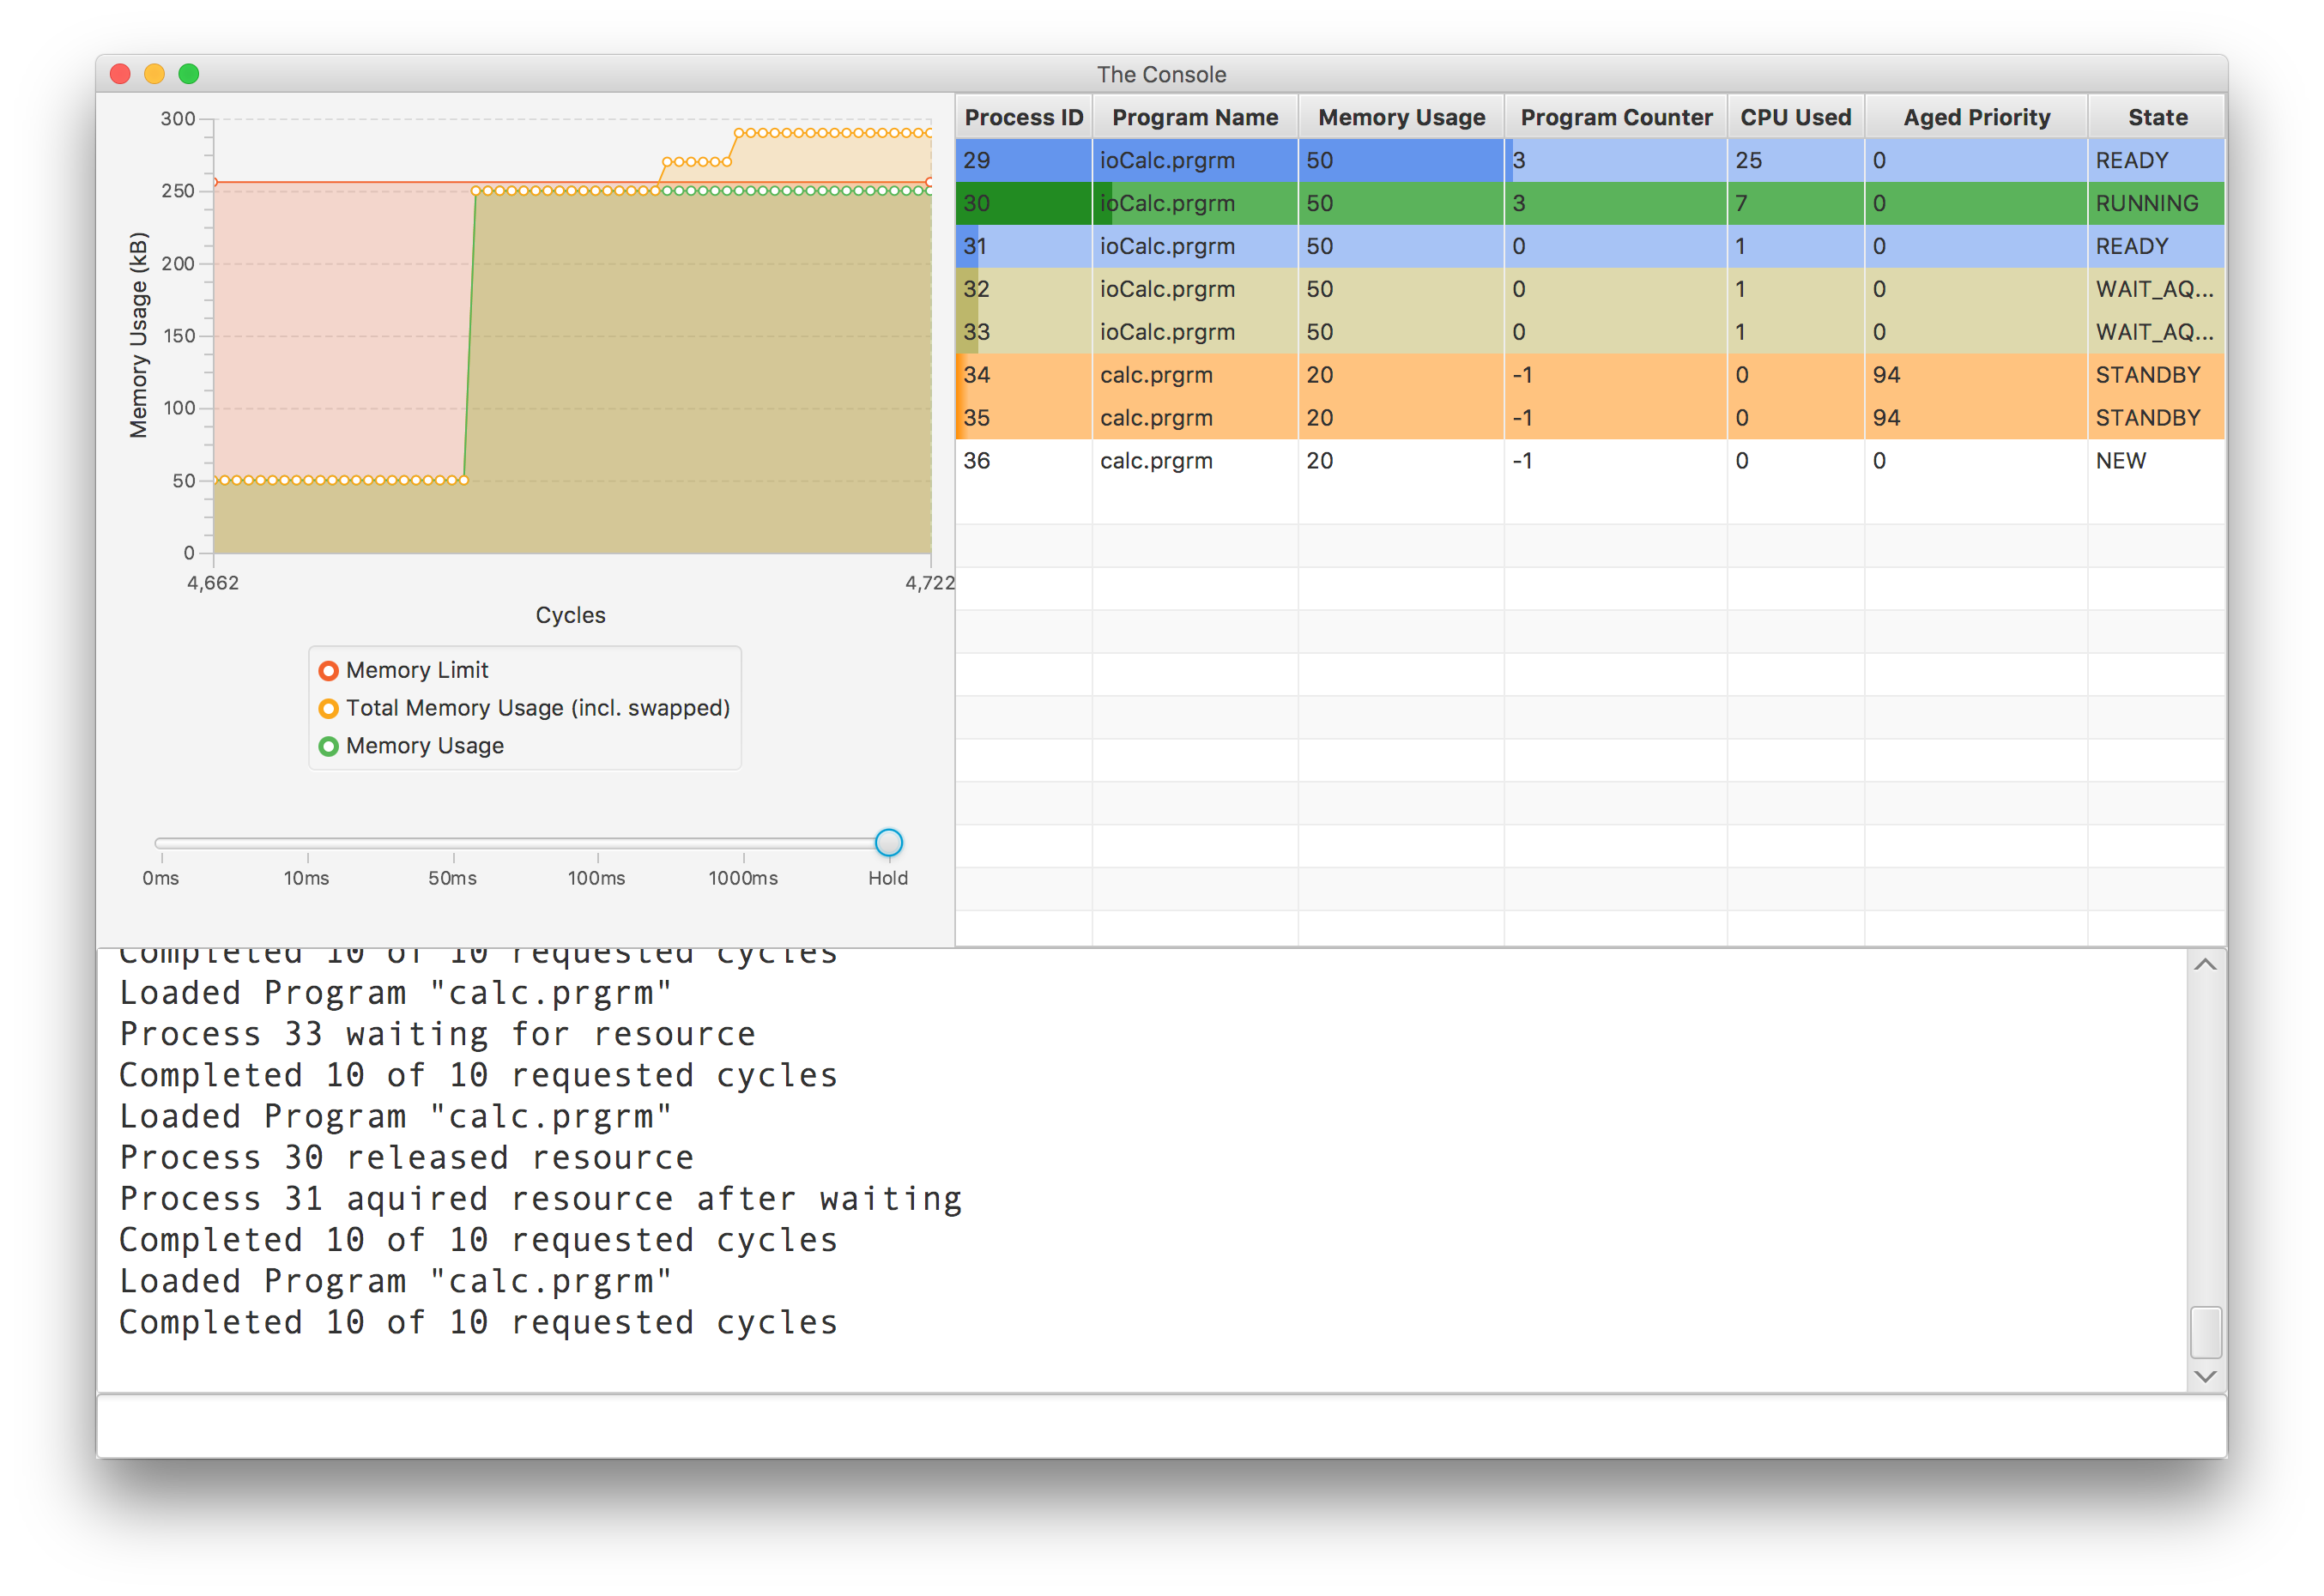
\includegraphics[width=\textwidth]{Demo.png}
\subsection{Overview}
The GUI features a live memory usage graph, process viewer, simulation speed control slider, and a terminal emulator for the simulated operating system. 


\subsection{Memory Graph}
The memory graph shows the system memory limit, the amount of memory currently being used, and the amount of total memory (including swapped out memory that isn't being used, but is ready to be swapped in by processes).
\begin{figure}[H]
  \centering
    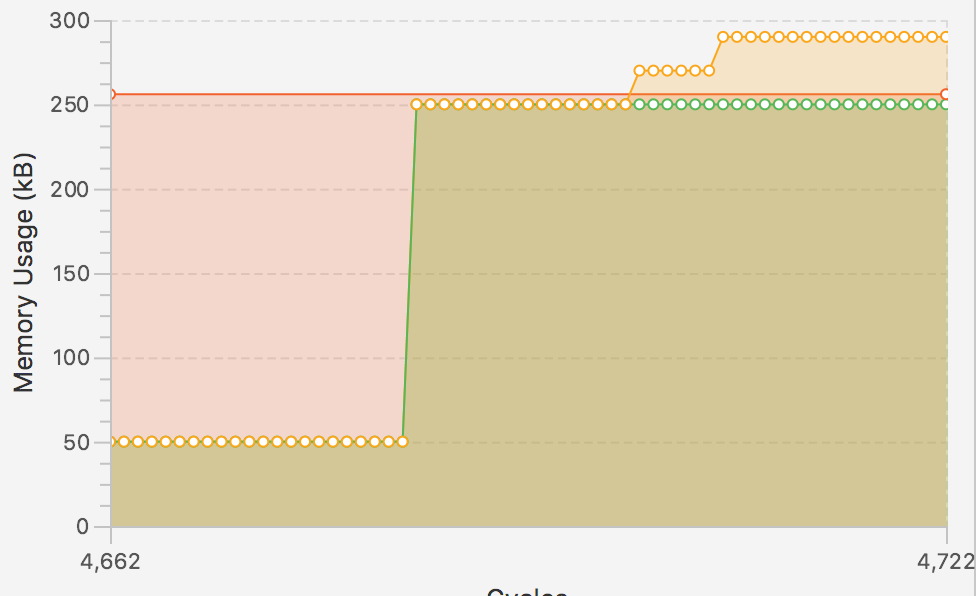
\includegraphics[scale=.5]{MemoryGraph.png}
  \caption{The memory graph showing that some processes are swapped out}
\end{figure}

\subsection{Delay Slider}
The slider changes the amount of delay between each CPU cycle. Moving this all the way to the right will temporarily pause execution. If the simulator is in the middle of an execution block, the block must be completely run before any other commands must be input. Thus, the slider may not be used to inject commands.

The slider can be used as a "step" button by quickly sliding from \textit{hold}, to \textit{1000ms}, and back to \textit{hold}.
\begin{figure}[H]
  \centering
    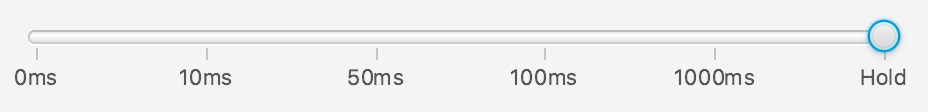
\includegraphics[scale=.5]{DelaySlider.png}
  \caption{The delay slider in the 'Hold' position}
\end{figure}

\subsection{Process Table}
The process table shows a complete list of processes, and is sortable by any column. Each row represents a process and is colored based on process state. The background color for each row also serves as a progress bar to hint at when the process will be finished executing.

\subsection{Terminal Emulator}
The terminal emulator supports the following commands: "PROC", "MEM", "LOAD", "EXE", "CAT", "RESET", and "EXIT".

Auto-suggest supports all commands, including parameters (file names) for LOAD and CAT. Auto-suggest even supports multiple parameters, and will not suggest file names that have already been typed.

\begin{figure}[H]
  \centering
    
\includegraphics[scale=.5]{AutoSuggest.png}
  \caption{\textit{test.prgrm} comes before \textit{test2.prgrm} in lexicographic order, but is not suggested because it is already used in a previous parameter }
\end{figure}

The terminal emulator supports the Enter key to repeat the last command, the Tab key to auto-complete suggestions, and the up and down arrow keys to browse command history.

If an typo is entered, the terminal emulator will try and figure out your desired command, and display it for you to type correctly.

\begin{figure}[H]
  \centering
    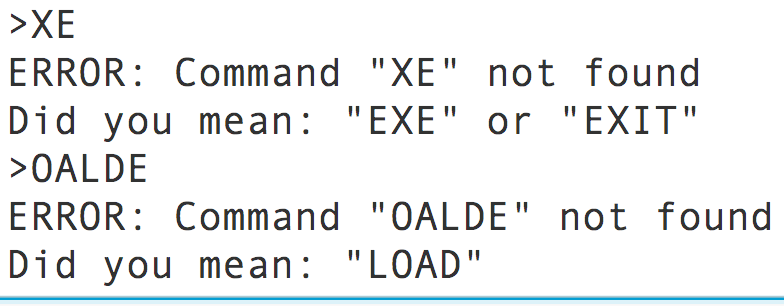
\includegraphics[scale=.5]{Typo.png}
  \caption{ \textit{EX} is similar to commands \textit{EXE} and \textit{EXIT}, so both are suggested}
\end{figure}

\begin{itemize}
	\item \textbf{PROC} is used to display info on all processes in plain-text. This is useful if you want to copy and paste process info, but is otherwise redundant (because of the process table)
	\item \textbf{MEM} is used to display the amount of memory currently being used, as well as the amount of memory that is swapped out.
	\item \textbf{LOAD}
		\begin{itemize}
			\item If no parameters are passed in, a list of loadable programs and jobs will be shown.
			\item One or more file names can be passed into be loaded by the simulator, in order of appearance. Job files are run on read, and are functionally equivalent to typing the contents of the job file into the terminal emulator.
		\end{itemize}
	\item \textbf{EXE} will run any program files that have been loaded. An integer can be passed in as a parameter to limit execution to a certain number of cycles. Otherwise, all loaded programs are run until termination.
	\item \textbf{CAT} behaves very similarly to its bash counterpart. If run without any parameters, some help text will be output to the terminal.
	\item \textbf{RESET} resets the simulator.
	\item \textbf{EXIT} exits the program.
\end{itemize}


\end{document}
